\section{Eigenanteil}

Mein Eigenanteil besteht darin, ein Java Programm zu erzeugen, welches eine Datei ver- und entschlüsseln kann. Geschrieben wurde es in Java mit der IDE Eclipse. Das Projekt besteht aus einem Paket, welches 8 verschiedene Klassen und 2 Interfaces enthält. Bei dem Projekt handelt es sich um ein Komandozeilenprogramm.\footnote{GitHub:  \url{https://github.com/Niffecs/JavaCrypt}} \\


Da das Programm keine Benutzeroberfläche hat, kann es nur schwer auf einer typischen IDE wie Netbeans oder Eclipse laufen. Der Grund dafür liegt in den (nach Netbeans benannten) Project Properties, in welchem der Nutzer Optionen angeben kann. Der folgende Abschnitt wird sich ausschließlich mit der CMD-Version beschäftigen. Auf UNIX Systemen läuft das Programm im Terminal (Bash) ebenfalls.\\

Anmerkung: Bei den meisten Computern befindet sich unter C:\ die Festplatte. Daher kann es sein, dass Windows etwas stört, denn er vergibt an dieser Stelle nur sehr ungern Schreibrechte. In dem Beispiel existiert das Laufwerk nur virtuell und ist somit nicht reell.
Für einen Test empfiehlt es sich, eine dummy Datei anzulegen. Ich nutze hier einfach eine test.txt Datei. Diese kann (und sollte) in dem Ordner liegen, in dem sich auch das Programm befindet. Es besteht auch eine andere Möglichkeit, allerdings würde dies die Arbeit nur erschweren. Die folgende Erstellung einer Datei mit Text ist in keinem Fall die solideste, aber dafür die einfachste.\\

\begin{center}
		\texttt{\textbf{C:\textbackslash > echo "Ich bin eine Testdatei" > test.txt}}
\end{center}

\subsection{MyCryptMain}
Nach dem erfolgreichen Erstellen der Datei kann ich nun beginnen. Die test.txt befindet sich in dem Ordner, den die CMD als Pfad angibt. Hier ist es das Laufwerk unter C:\.
Nach dem Aufruf erscheint folgende Ausgabe mit dem Ende des Programmes.
\begin{center}
	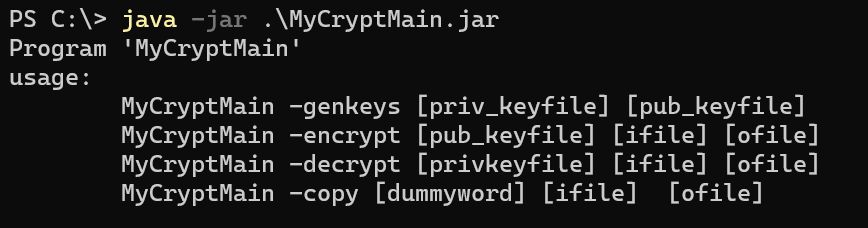
\includegraphics{./img/basic}
	\captionof{figure}{\label{fig:basic}MyCrypt Menü}
\end{center}
Das Java Programm wurde als Semi.jar kompiliert. In diesem Zustand ist es von jedem „normalen“ Betriebssystem aus startbar. Es erklärt sich von selbst, dass Objekte wie -genkeys, -encrypt, -decrypt und -copy als Optionen fungieren und einfach nur angehängt werden. \\
Die Attribute, welche in den eckigen Klammern stehen, sind zu einem Teil optional und zu einem anderen Teil erforderlich. Ich werde nun alle Optionen Schritt für Schritt erklären.

\subsection{Erzeugung von Schlüsseln}
Die Option -genkeys ist für die Schlüsselverwaltung zuständig. Sie hat zwei Attribute, welche den Pfad zu dem Schlüsselpaar angeben. Dabei ist in priv\_keyfile der Pfad zu dem privaten Schlüssel und in dem Attribut pub\_keyfile der Pfad zu dem öffentlichen Schlüssel hinterlegt. Dies sind freiwillige Angaben. Sollte einer der Pfade fehlen, wird eine entsprechende *.key Datei angelegt. Für den Privaten Schlüssel ergibt sich dann der Pfad aus der Lage der jar Datei. In dem Ordner, wo er sich befindet, werden nun die Schlüssel abgelegt. Der private Schlüssel als priv.key und der öffentliche Schlüssel als pub.key.\\ Ich empfehle für keinen Schlüssel einen Pfad anzugeben, da dies die Verwaltung einfacher macht. Die Lese und Schreibrechte in dem entsprechenden Ordner wird vorausgesetzt. Daraus ergibt sich folgende Ausgabe.\\

\begin{center}
	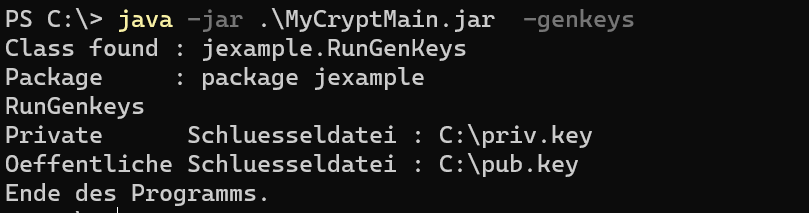
\includegraphics[width=\textwidth]{./img/genkeys}
	\captionof{figure}{\label{fig:genkeys}MyCrypt genkeys}
\end{center}

Auf die angegebene Klasse RunGenKeys sowie auf das package jexample und dessen großartigen Namen werde ich später noch genauer eingehen. Die Ausgabe suggeriert dem Nutzer den Pfad, wo die Schlüssel abgelegt werden. Als kleine Info: Die Schlüssel werden auf BASE64 gespeichert, was das Öffnen etwas lustig macht. Man kann sich den Schlüssel nicht einfach als Wert oder String vorstellen, sondern mehr als abstraktes Gebilde. Eine tiefgreifendere Bearbeitung der Schlüssel ist auf Grund des begrenzten Umfanges der Seminararbeit nicht möglich. \\


\subsection{Verschlüsseln von Datein}
Die zweite Option ist die –encrypt, welche für die Verschlüsselung zuständig ist. Dazu benötigt sie den öffentlichen Schlüssel, welcher als pub\_keyfile bezeichnet wird. Diese Angabe ist für die Verschlüsselung zwingend erforderlich. Die ifile, besser bekannt als Inputfile, bezeichnet die Datei, die verschlüsselt werden soll. Das der Pfad zu dieser angegeben werden muss, liegt ebenfalls auf der Hand. Dabei ist es irrelevant, in welchem Datentyp die Datei vorliegt.\\
 Das ofile steht an dieser Stelle für die Outputfile. Die Angabe von diesem Wert ist obligatorisch und es steht dem Nutzer somit frei, einen Eintrag zu tätigen. Sollte keine Eingabe gemacht worden sein, erfolgt die Ausgabe in einer encr\_outp.dat Datei. Dat steht hier als Dateiendung für Datei.\\


\begin{center}
	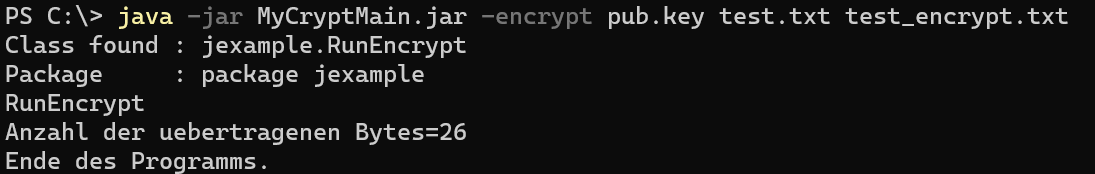
\includegraphics[width=\textwidth]{./img/encrypt}
	\captionof{figure}{\label{fig:encrypt}MyCrypt encrypt}
\end{center}
Hier fällt auf, dass zwar dasselbe Package genutzt wurde, jedoch eine andere Klasse. Grundlegend kann man sagen, dass je nach Befehl, eine andere Klasse genutzt wird. Näheres dazu werde ich später kurz beschreiben. Das Programm gibt uns die Anzahl der Bytes an, die übertragen wurden. In unserem Fall wären das 54 Bytes. Da die Datei sehr klein ist, geht auch die Datei sehr schnell von statten. Danach erfolgt wieder die Beendigung des Programmes, denn für jeden anderen Auftrag muss ein anderer Befehl genutzt werden. \\

\subsection{Entschlüsseln von Datein}
Wie bereits aus der Arbeit hervorgegangen ist, wird zum Entschlüsseln der private Schlüssel genutzt, welcher ebenfalls angegeben werden muss. Ich empfehle ausdrücklich, auch hier alle Attribute mitzuführen, da ich mir so aussuchen kann, unter welchem Namen bzw. Dateiformat die entschlüsselte Datei gespeichert wird. Bei dieser Funktion ist die Input Datei, die Datei, welche bereits verschlüsselt wurde.\\


\begin{center}
	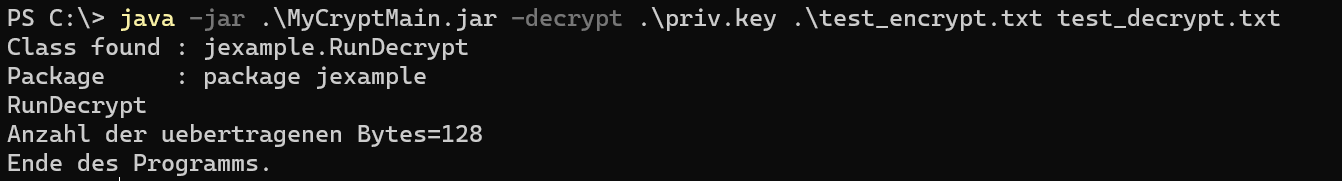
\includegraphics[width=\textwidth,height=4cm]{./img/decrypt}
	\captionof{figure}{\label{fig:decrypt}MyCrypt decrypt}
\end{center}

Nach dem erfolgreichen Aufruf dieser Methode wird die Datei wieder entschlüsselt. Dabei werden mehr Bytes übertragen als bei der Verschlüsselung.
In der Datei test.txt befindet sich derselbe Inhalt wie in der Datei test\_decrypt.txt. Es ist selbsterklärend, dass, wenn ich eine Datei mit einem öffentlichen Schlüssel verschlüssele, auch den dazugehörigen öffentlichen Schlüssel nutze, um die Datei wieder zu entschlüsseln.

\subsection{UML - Diagramm}
\begin{center}
	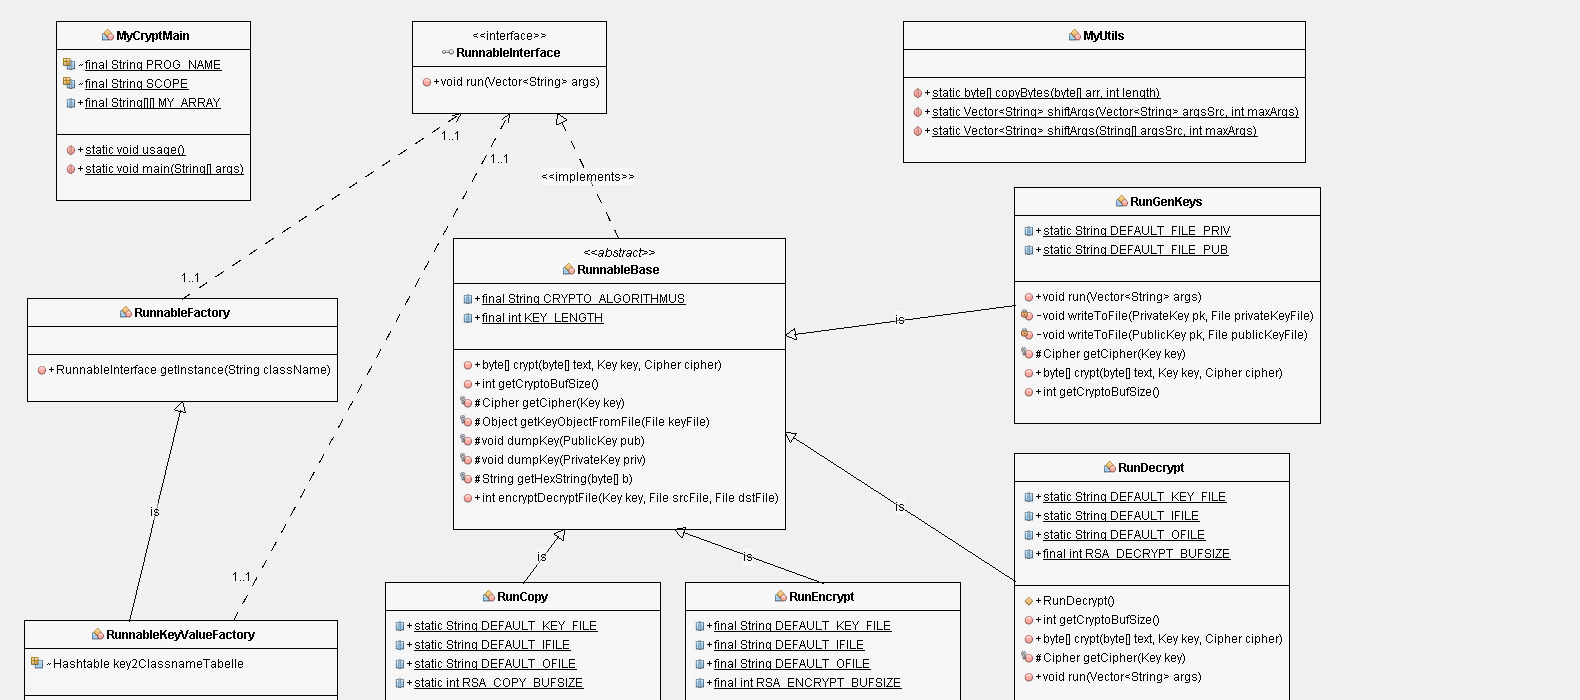
\includegraphics[width=1\textwidth]{./img/UML}
	\captionof{figure}{\label{fig:uml} UML Diagramm}
\end{center}